\chapter{Поиск и объединённая система (ЛР4, РК1)}

\section{Постановка задачи}

Рекомендательная система отвечает на вопрос <<что ещё мне может понравиться>>. Пользователь, который знает, что ему нужно, формулирует ограничения сам вроде <<травяной, не крепче 30\,\%, итальянский>>. ЛР4 добавляет такой \textbf{параметрический поиск}. Пользователь задаёт ограничения по фильтрам, любую их часть, и получает выборку подходящих объектов. Если выборка пуста, система не должна отвечать пустым экраном. Она выдаёт объекты с формулировкой <<не найдено точного соответствия, однако, возможно, Вам понравится>>.

РК1 объединяет поиск и рекомендации в одну систему с общим интерфейсом. Нужно фильтровать полученные рекомендации и хранить историю запросов. Тогда можно уточнять результат предыдущего поиска или запроса рекомендаций либо начинать заново. Работа идёт по циклу <<поиск $\rightarrow$ рекомендации $\rightarrow$ поиск $\rightarrow$ \ldots>>.

\section{Выбор фильтров}

Набор фильтров повторяет то, что пользователь видит в каталогах крупных интернет-магазинов. Это категория, у нас дерево вкусов, бренд, страна, числовые диапазоны вместо цены, характеристики-флаги и строка поиска по названию. Каждый признак датасета из ЛР1, кроме служебных, представлен фильтром подходящего типа в таблице~\ref{tab:lr4_filters}.

\begin{table}[H]
	\centering
	\caption{Фильтры поиска}
	\label{tab:lr4_filters}
	\footnotesize\setlength{\tabcolsep}{4pt}
	\begin{tabular}{|L{2.7cm}|L{2.7cm}|L{4.1cm}|c|L{2.5cm}|}
		\hline
		Фильтр & Элемент формы & Степень соответствия $\deg_f(x)$ & Вес $w_f$ & Ослабление \\ \hline
		Название & строка & 1 за подстроку, иначе нечёткое совпадение $\geq 0{,}7$ или 0 & 3 & снять \\ \hline
		Вкус & дерево с флажками L1, L2, L3 & доля общего пути с ближайшим выбранным узлом & 3 & подняться к родителю \\ \hline
		Крепость, сахар & <<от>> и <<до>> & 1 внутри, линейно до 0 при выходе на 25\,\% размаха & 2 & расширить на 10\,\% размаха \\ \hline
		Горечь & да / нет / неважно & 1 или 0 & 1,5 & снять \\ \hline
		Класс сладости & флажки термов & $1 - $ расстояние до ближайшего терма$/3$ & 1 & добавить соседние термы \\ \hline
		Дерево, страна, производитель & переключатель, флажки & 1 или 0 & 1 & снять \\ \hline
		Объём & <<от>> и <<до>> & как у крепости & 0,5 & расширить \\ \hline
	\end{tabular}
\end{table}

\textbf{Семантика запроса.} Разные фильтры объединяются конъюнкцией, то есть логическим И. Значения внутри одного фильтра объединяются дизъюнкцией, например <<Франция или Италия>> и <<амаро или кройтер>>. Незаданный фильтр ограничений не накладывает, а пустой запрос возвращает весь каталог. Такая семантика привычна по интернет-магазинам. Запрос --- конъюнкция фильтров.

Принятые решения по отдельным фильтрам приведены ниже.
\begin{itemize}[leftmargin=1.6\parindent, label*=---]
	\item \textbf{Вкус задаётся узлами дерева, а не только листьями.} Выбор узла <<Травяные>> включает всё поддерево. Пользователь может быть точным и выбрать <<амаро>> или общим и выбрать <<что-нибудь травяное>>, не отмечая все листья вручную.
	\item \textbf{Текстовый поиск} не учитывает регистр и диакритику. Запрос <<KAHLUA>> находит <<Kahl\'ua>>, а <<creme>> --- <<Cr\`eme>>. При опечатке включается нечёткое совпадение по коэффициенту \code{difflib.SequenceMatcher}. Например, <<kalua>> находит Kahl\'ua со степенью 0,8. Порог 0,7 отсекает случайные совпадения. Без него <<kalua>> получал степень 0,6 с девятью посторонними объектами.
	\item \textbf{Сладость доступна двумя способами.} Это точный диапазон в граммах на литр и слова через лингвистическую переменную из ЛР1. Покупатель редко знает содержание сахара в граммах.
\end{itemize}

\section{Проверка корректности ввода}

Каждое поле формы проверяется независимо. Ошибки всех полей собираются в один ответ, чтобы пользователь исправил всё за один раз. Проверяется следующее.
\begin{itemize}[leftmargin=1.6\parindent, label*=---]
	\item Числа диапазонов. Допускается и десятичная запятая, и точка. Строки <<10x>>, <<nan>> и <<inf>> отклоняются регулярным выражением.
	\item Физические границы. Крепость от 0 до 100\,\%, сахар от 0 до 1000 г/л, объём от 0,05 до 5 л. Значение <<от>> не больше значения <<до>>.
	\item Узлы вкуса, страны, производители и термы. Принимаются только значения из справочников каталога.
	\item Трёхзначные флаги принимают только \code{any}, \code{yes} и \code{no}. Длина строки поиска не больше 100 символов. Типы полей проверяются явно.
\end{itemize}
Границы, выходящие за значения датасета, но физически возможные, ошибкой не считаются. Крепость 60\,\% физически возможна, хотя в датасете её нет. Такой запрос просто не найдёт точных совпадений, и сработает механизм из раздела~\ref{sec:lr4_fallback}.

\section{Пустая выдача: <<возможно, Вам понравится>>}
\label{sec:lr4_fallback}

\subsection{Рассмотренные подходы}

Задание допускает два пути. Можно использовать механизм рекомендаций или отодвинуть слишком строгие границы фильтров.
\begin{enumerate}[leftmargin=1.6\parindent]
	\item \textbf{Рекомендации по профилю.} Не подходят как основной механизм. У пользователя может не быть ни одного лайка, а рекомендации не учитывают сам запрос.
	\item \textbf{Ослабление фильтров} по схеме query relaxation~\cite{jannach2009}. Реализован жадный алгоритм \code{RelaxationAdvisor}. На каждом шаге пробуется ослабить каждый фильтр на один шаг из таблицы~\ref{tab:lr4_filters}. Выбирается вариант, который даёт точные совпадения, а при их отсутствии сильнее всего повышает лучшую степень соответствия. При равенстве выбирается вариант с меньшей ценой. Ценой считается вес фильтра, а для расширения --- половина веса. Подход объясним и говорит <<ослабьте крепость до 19\,\%>>. Однако он выдаёт только объекты, прошедшие ослабленный запрос. Ослабленное ограничение снимается целиком для всех объектов, даже если искомый объект нарушал другое.
	\item \textbf{Функция полезности} как мягкие ограничения~\cite{mcsherry2003}. Каждый объект получает степень соответствия запросу
	\begin{equation}
		U(x) = \frac{\sum_f w_f \deg_f(x)}{\sum_f w_f},
		\label{eq:lr4_utility}
	\end{equation}
	Это очки за выполненные фильтры и штраф за нарушенные. Штраф пропорционален расстоянию до границы. Объекты ранжируются по $U(x)$. Нарушение на 1\,\% крепости почти не штрафуется, а нарушение на 20\,\% --- полностью. Нарушение узла вкуса оценивается по общему пути в дереве, как в мере ЛР2. <<Кройтер>> вместо <<амаро>> получает 2/3.
\end{enumerate}

\subsection{Сравнение стратегий}

Использован протокол <<восстановления задуманного объекта>>. Для каждого ликёра $x$ строится запрос из его группы L2, класса сладости и флага дерева. Затем два ограничения из четырёх портятся. Крепость сдвигается на 3--8 п.\,п., сахар --- на 20--60 г/л, страна заменяется, а горечь инвертируется. В результате точных совпадений нет. Так моделируется пользователь, который неточно помнит параметры. Получено 179 сценариев из 6 пар искажений для 30 объектов без сценариев, где точные совпадения остались. Метрика Hit($k$) --- доля сценариев, в которых $x$ оказался среди первых $k$.

\begin{table}[H]
	\centering
	\caption{Восстановление задуманного объекта при пустой выдаче. Всего 179 сценариев}
	\label{tab:lr4_fallback}
	\footnotesize
	\begin{tabular}{|L{6.5cm}|c|c|}
		\hline
		Стратегия & Hit(1) & Hit(5) \\ \hline
		ослабление фильтров, выдача по ослабленному запросу & 0,603 & 0,698 \\ \hline
		\textbf{функция полезности $U(x)$} & \textbf{0,637} & \textbf{1,000} \\ \hline
	\end{tabular}
\end{table}

Функция полезности ни разу не потеряла задуманный объект из первой пятёрки, что видно из таблицы~\ref{tab:lr4_fallback}. Ослабление теряет его в 30\,\% сценариев. Жадный алгоритм снимает ограничение, которое мешало другому объекту, и выдача уходит в сторону. В 8,9\,\% сценариев ослабление предлагало расширить вкус, то есть самое важное ограничение. Поэтому принято комбинированное решение. \textbf{Выдача <<возможно, Вам понравится>> ранжируется функцией полезности}, а результат \code{RelaxationAdvisor} показывается как подсказка. Пользователь видит, какие ограничения достаточно ослабить, чтобы появились точные совпадения, и сколько их будет, как на рисунке~\ref{fig:ui_lr4_fallback}. Рядом с каждым объектом указываются невыполненные фильтры и степень их выполнения.

\section{Объединённая система (РК1)}

\subsection{Сценарий работы}

Объединённая система в каталоге \code{4-search} использует рекомендательное ядро ЛР3 без копирования. Пакет \code{recsys} подключается из каталога \code{3-likesdislikes} как есть. Сценарий работы показан на рисунке~\ref{fig:rk1_cycle}.
\begin{itemize}[leftmargin=1.6\parindent, label*=---]
	\item \textbf{Поиск} --- новый запрос фильтров по всему каталогу.
	\item \textbf{Лайк и дизлайк} доступны на любой карточке любой выдачи. Профиль хранится в сессии и не теряется между шагами.
	\item \textbf{Рекомендации} строятся по профилю сессии. Версия выбирается автоматически. Одна затравка --- v1, только лайки --- v2, есть дизлайки --- v3. Область рекомендаций --- весь каталог или текущая выдача по принципу <<порекомендуй среди найденного>>. Флажок <<отфильтровать рекомендации>> применяет фильтры формы к рекомендациям.
	\item \textbf{Уточнение} применяет фильтры к результатам текущего шага и сохраняет их порядок и объяснения.
	\item \textbf{История} сохраняет каждый шаг. Щелчок по шагу возвращает его результат и восстанавливает форму фильтров. После этого уточнять можно уже от него. Кнопки <<Начать заново>> и <<Сбросить всё>> начинают работу с чистого листа. Первая очищает историю, но оставляет профиль.
\end{itemize}

\begin{figure}[H]
	\centering
	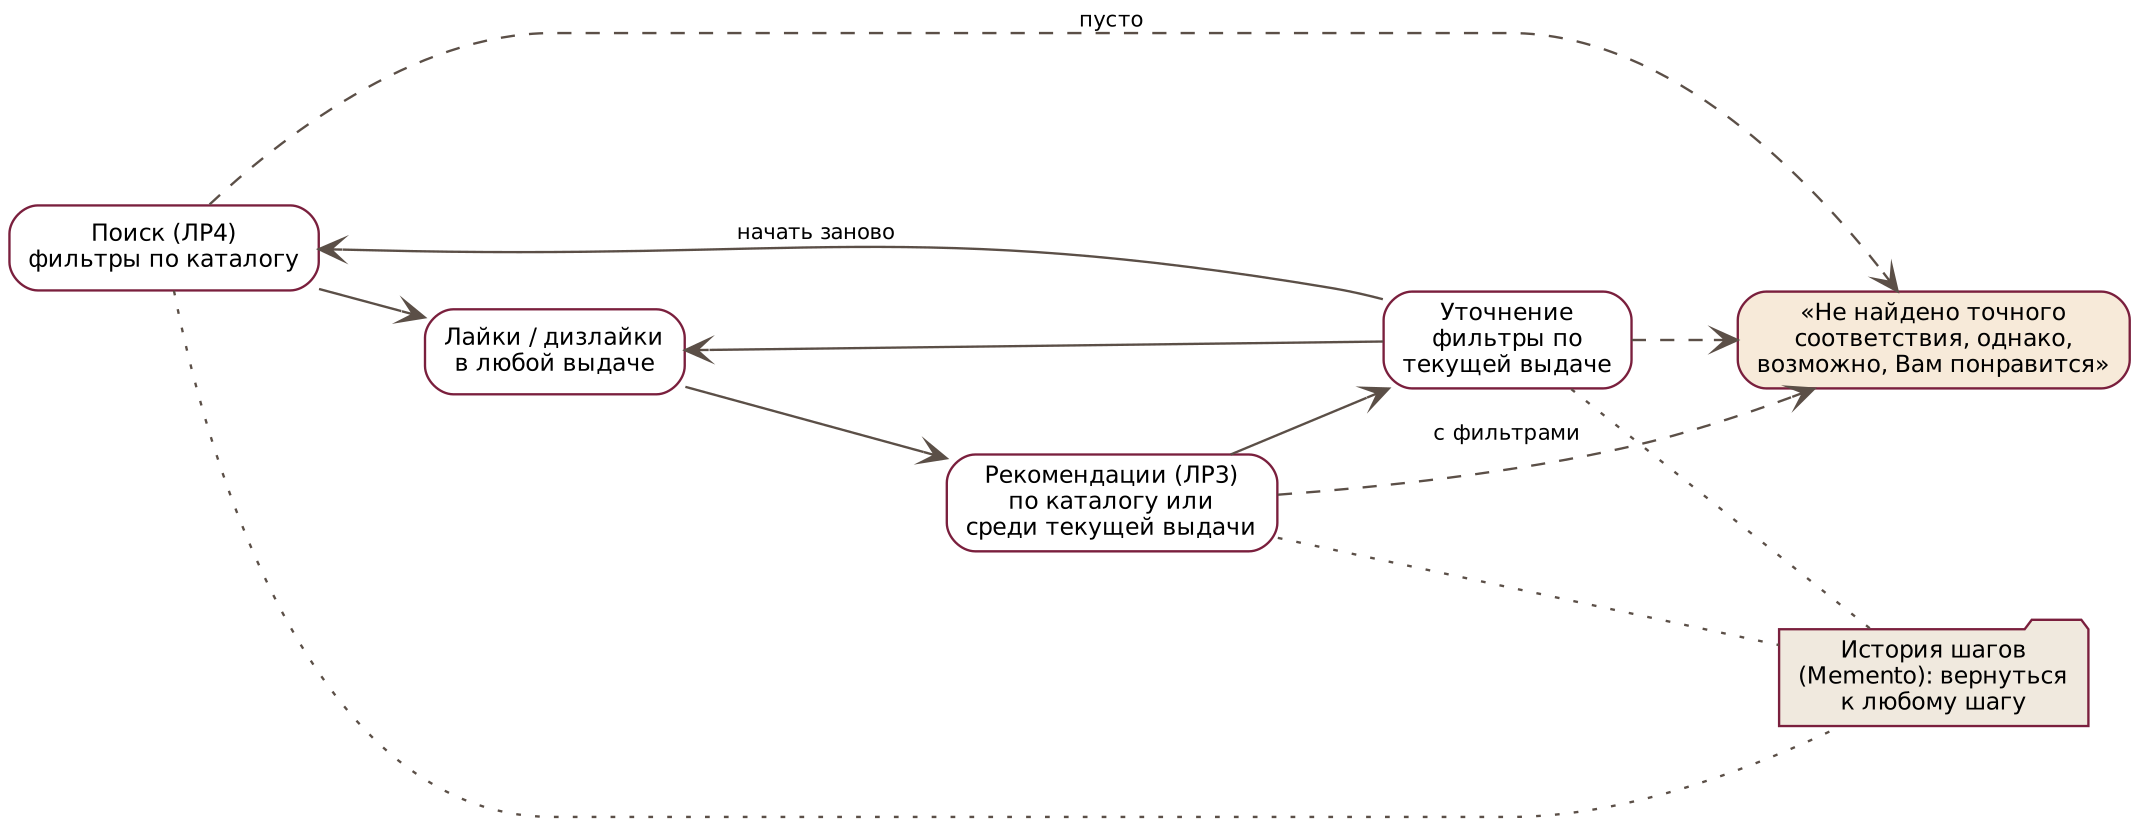
\includegraphics[width=\textwidth]{diags/cycle.png}
	\caption{Цикл работы объединённой системы}
	\label{fig:rk1_cycle}
\end{figure}

\subsection{Функция полезности для фильтрации рекомендаций}

Когда фильтруются рекомендации, у объекта две оценки. Это релевантность рекомендателя $r(x)$ и степень соответствия фильтрам $U(x)$. Итоговая полезность
\begin{equation}
	S(x) = U(x)\cdot\bigl((1-\lambda) + \lambda\, r(x)\bigr), \qquad \lambda = 0{,}5.
	\label{eq:rk1_score}
\end{equation}
Если есть точные совпадения с $U = 1$, они показываются в порядке рекомендателя. Порядок групп интересов из ЛР3 при этом сохраняется. Если точных совпадений нет, объекты ранжируются по $S(x)$. Выбрано произведение, а не сумма. Объект должен быть хорош по обоим критериям, и сильная рекомендация не компенсирует полное нарушение фильтров. При $U = 0$ значение $S$ тоже равно нулю. При $\lambda = 0{,}5$ релевантность может изменить оценку не более чем вдвое. Фильтры остаются главными, потому что пользователь задал их явно. Рекомендации же упорядочивают объекты внутри одинаково подходящих.

\section{Пользовательский интерфейс}

Экран разделён на три колонки. Слева форма фильтров, в центре выдача текущего шага, справа профиль, параметры рекомендаций и история. Ниже показан сквозной сценарий.

На рисунке~\ref{fig:ui_lr4_search} показан поиск по фильтрам <<фруктовые, крепость 20--30\,\%>>.

\begin{figure}[H]
	\centering
	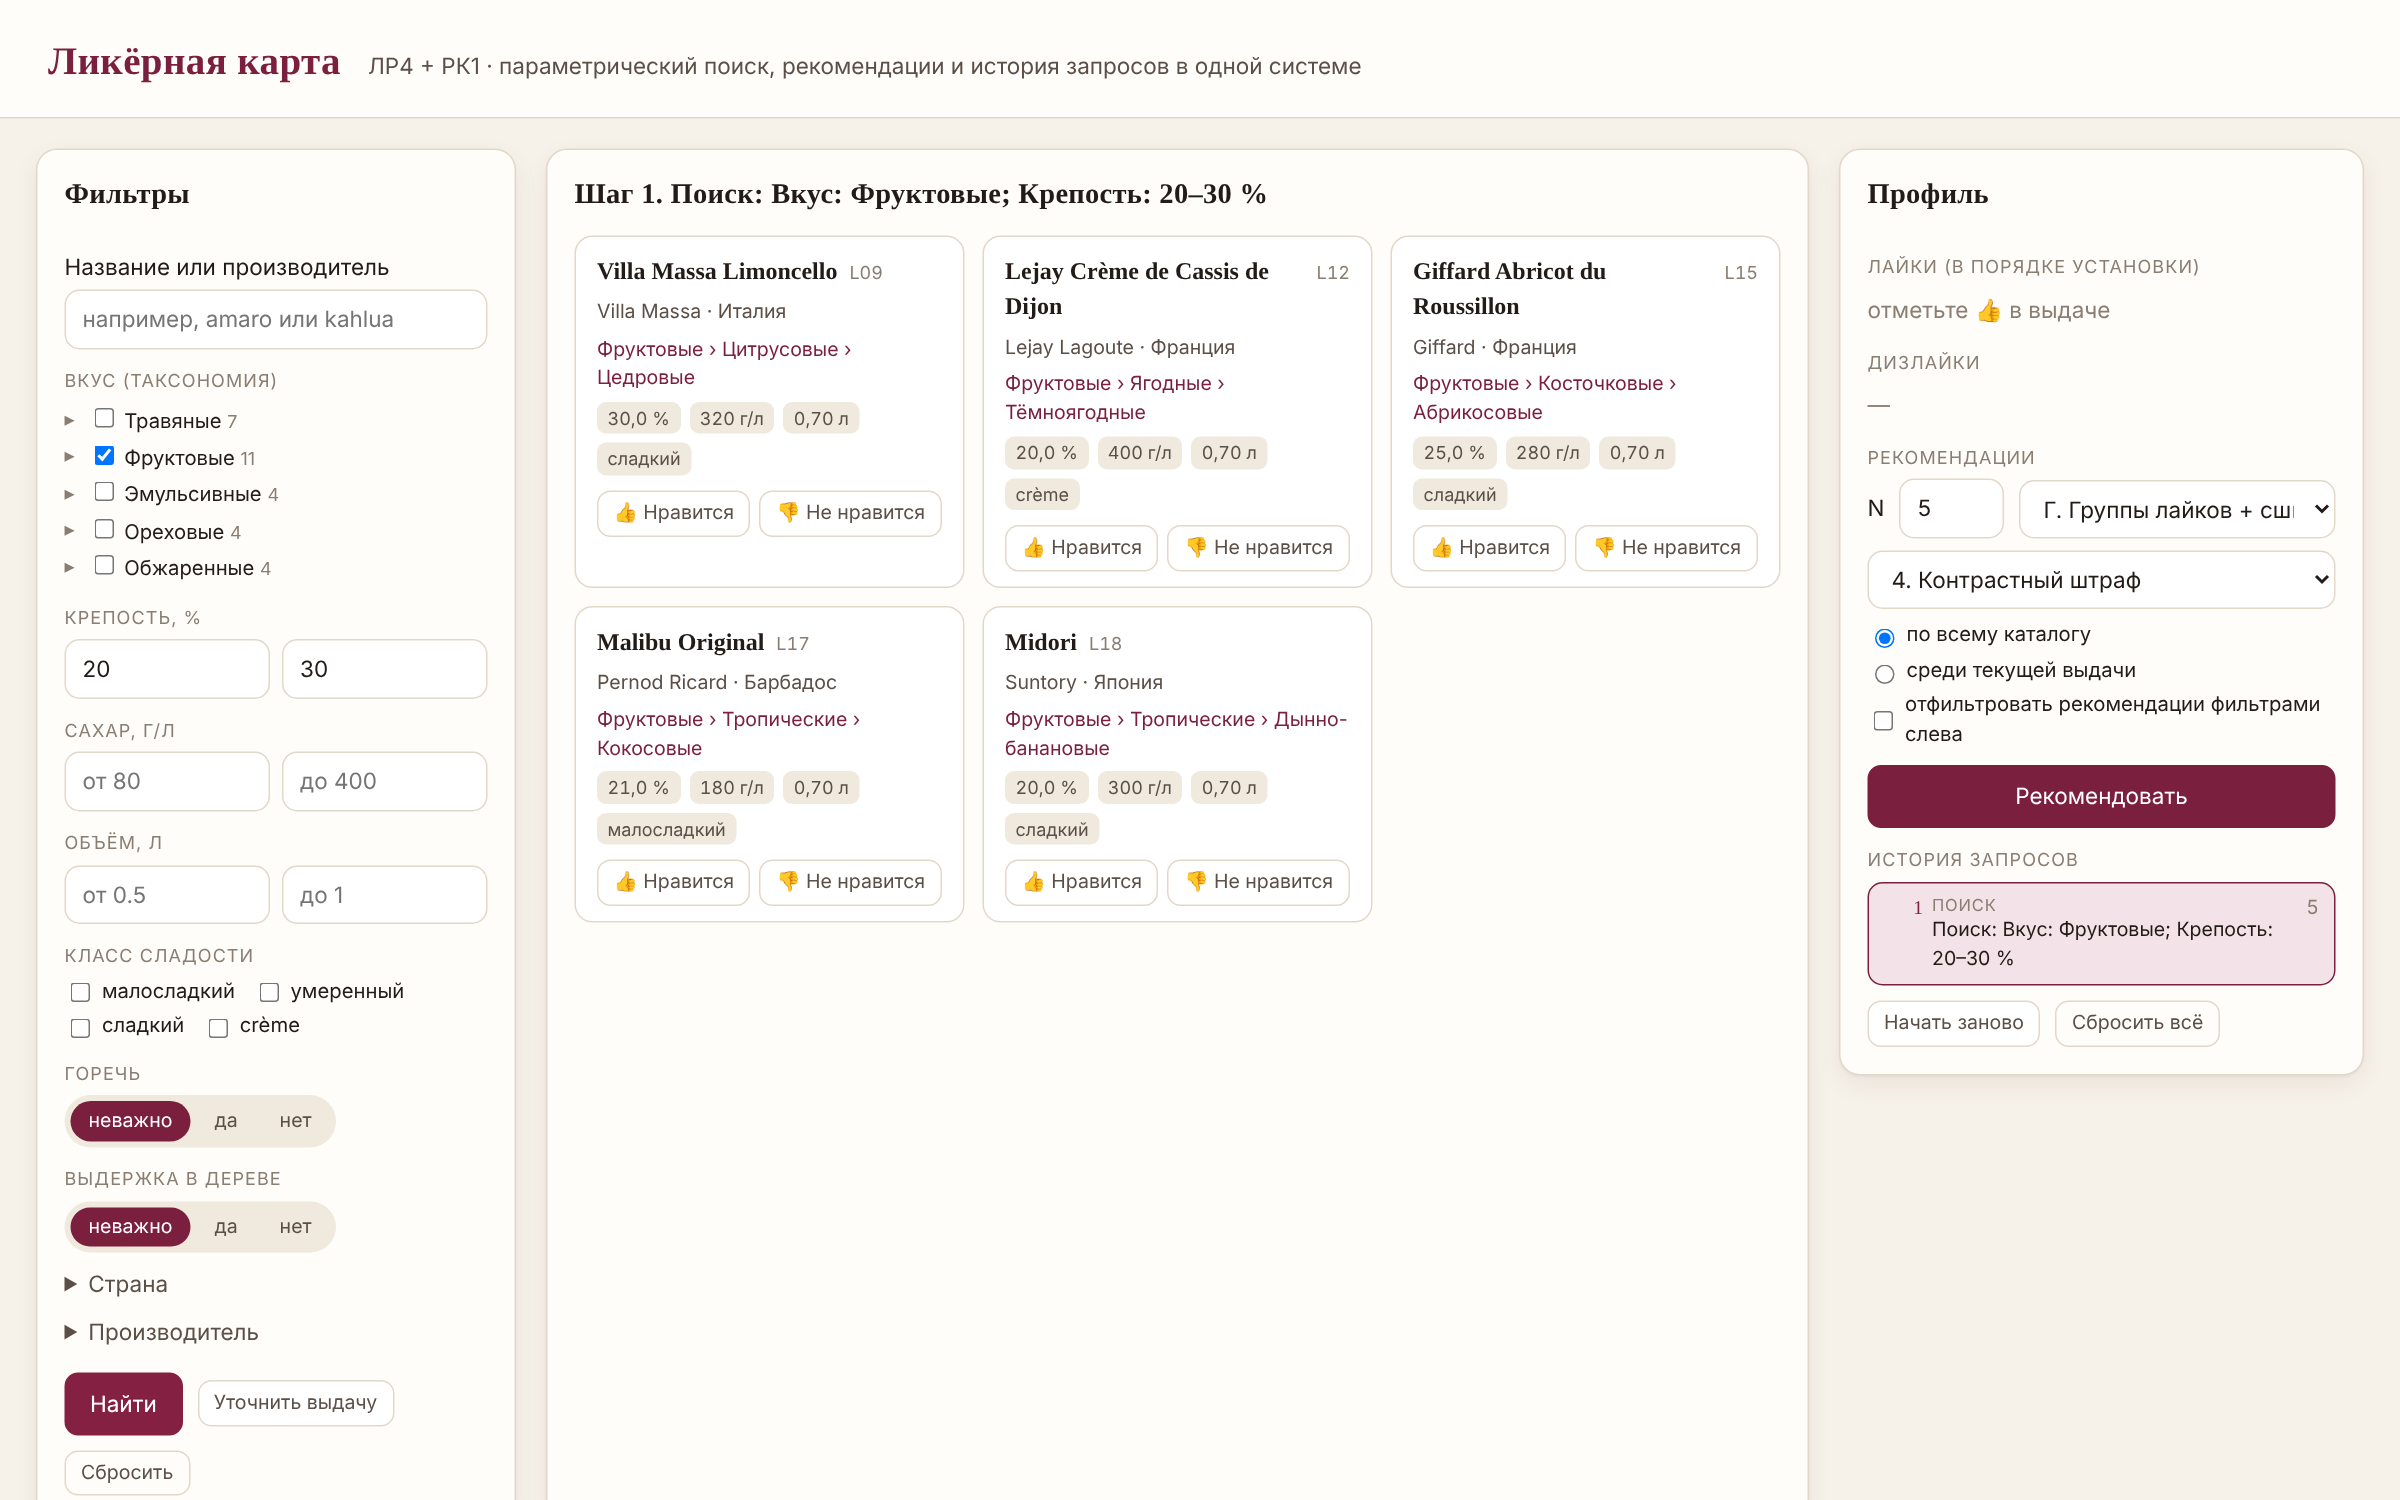
\includegraphics[width=\textwidth]{ui/lr4_search.png}
	\caption{Шаг 1. Поиск фруктовых ликёров крепостью 20--30\,\%}
	\label{fig:ui_lr4_search}
\end{figure}

На рисунке~\ref{fig:ui_lr4_fallback} точных совпадений нет. Объекты ранжированы функцией полезности, у каждого указаны невыполненные фильтры. Подсказка предлагает снять горечь и расширить крепость до 19\,\%.

\begin{figure}[H]
	\centering
	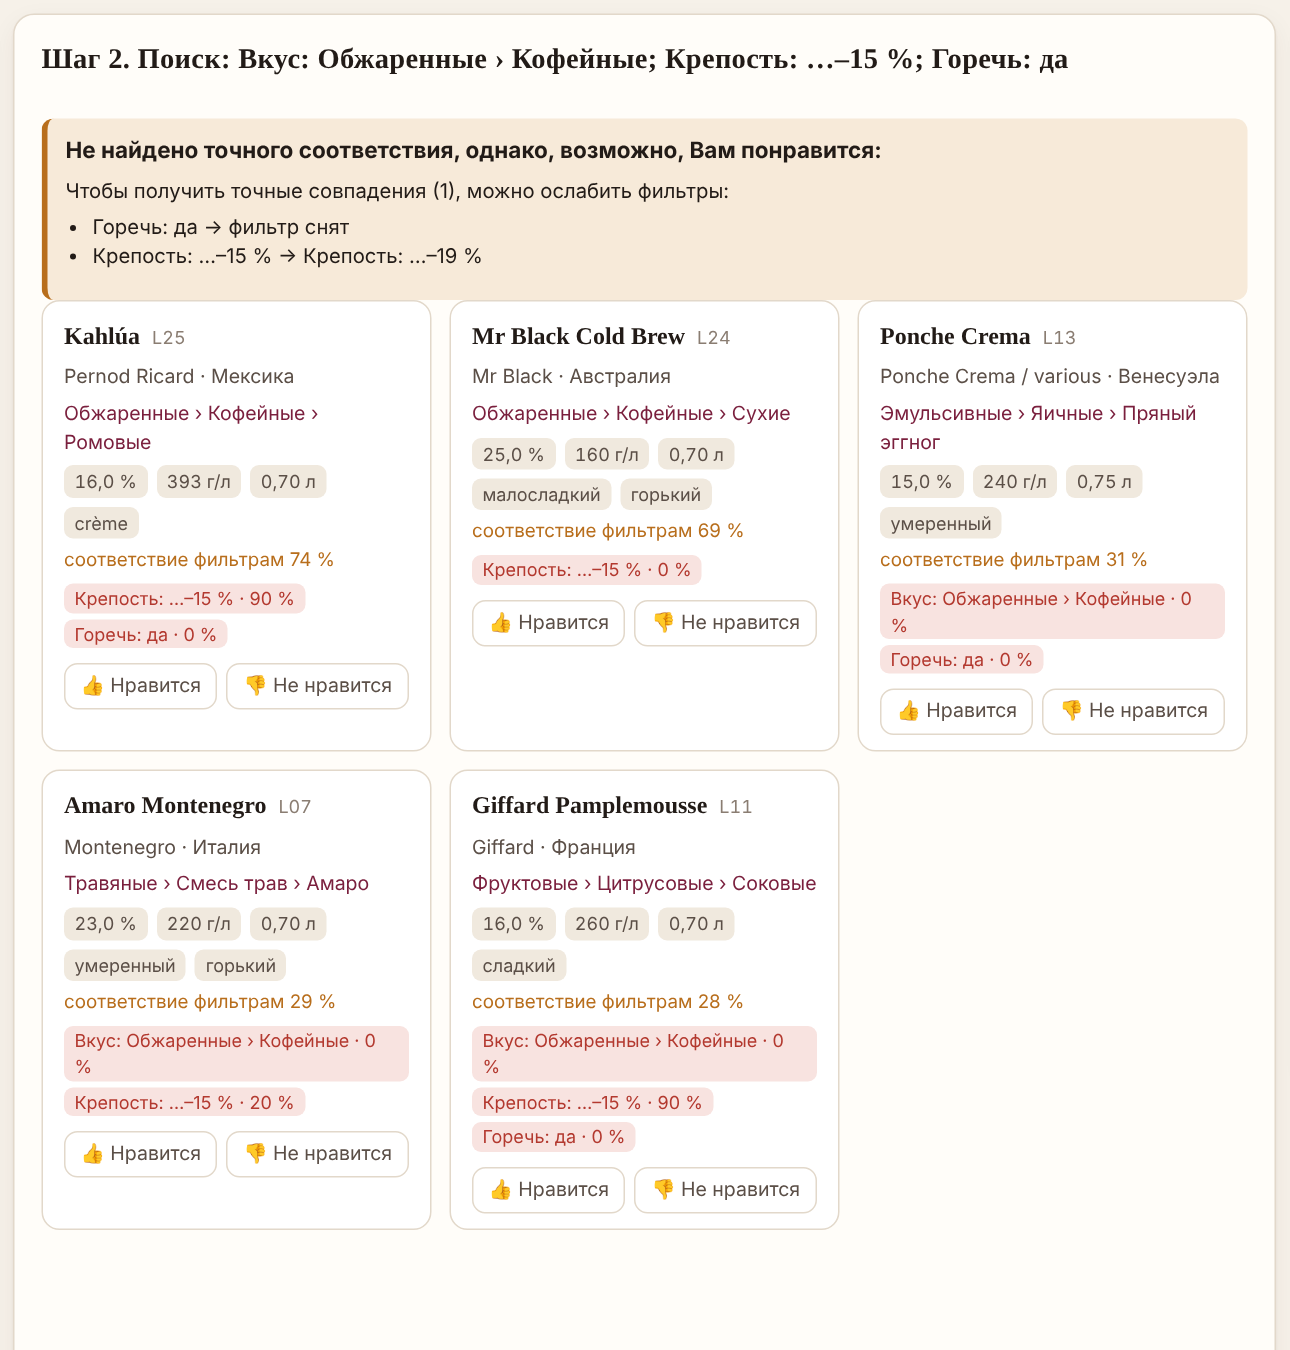
\includegraphics[width=0.66\textwidth]{ui/lr4_fallback.png}
	\caption{Шаг 2. Пустая выдача для запроса <<кофейные, не крепче 15\,\%, горькие>>. Ранжирование функцией полезности, невыполненные фильтры и подсказка ослабления}
	\label{fig:ui_lr4_fallback}
\end{figure}

На рисунке~\ref{fig:ui_lr4_rec} пользователь поставил два лайка и один дизлайк прямо на карточках выдачи. Справа построены рекомендации версии v3.

\begin{figure}[H]
	\centering
	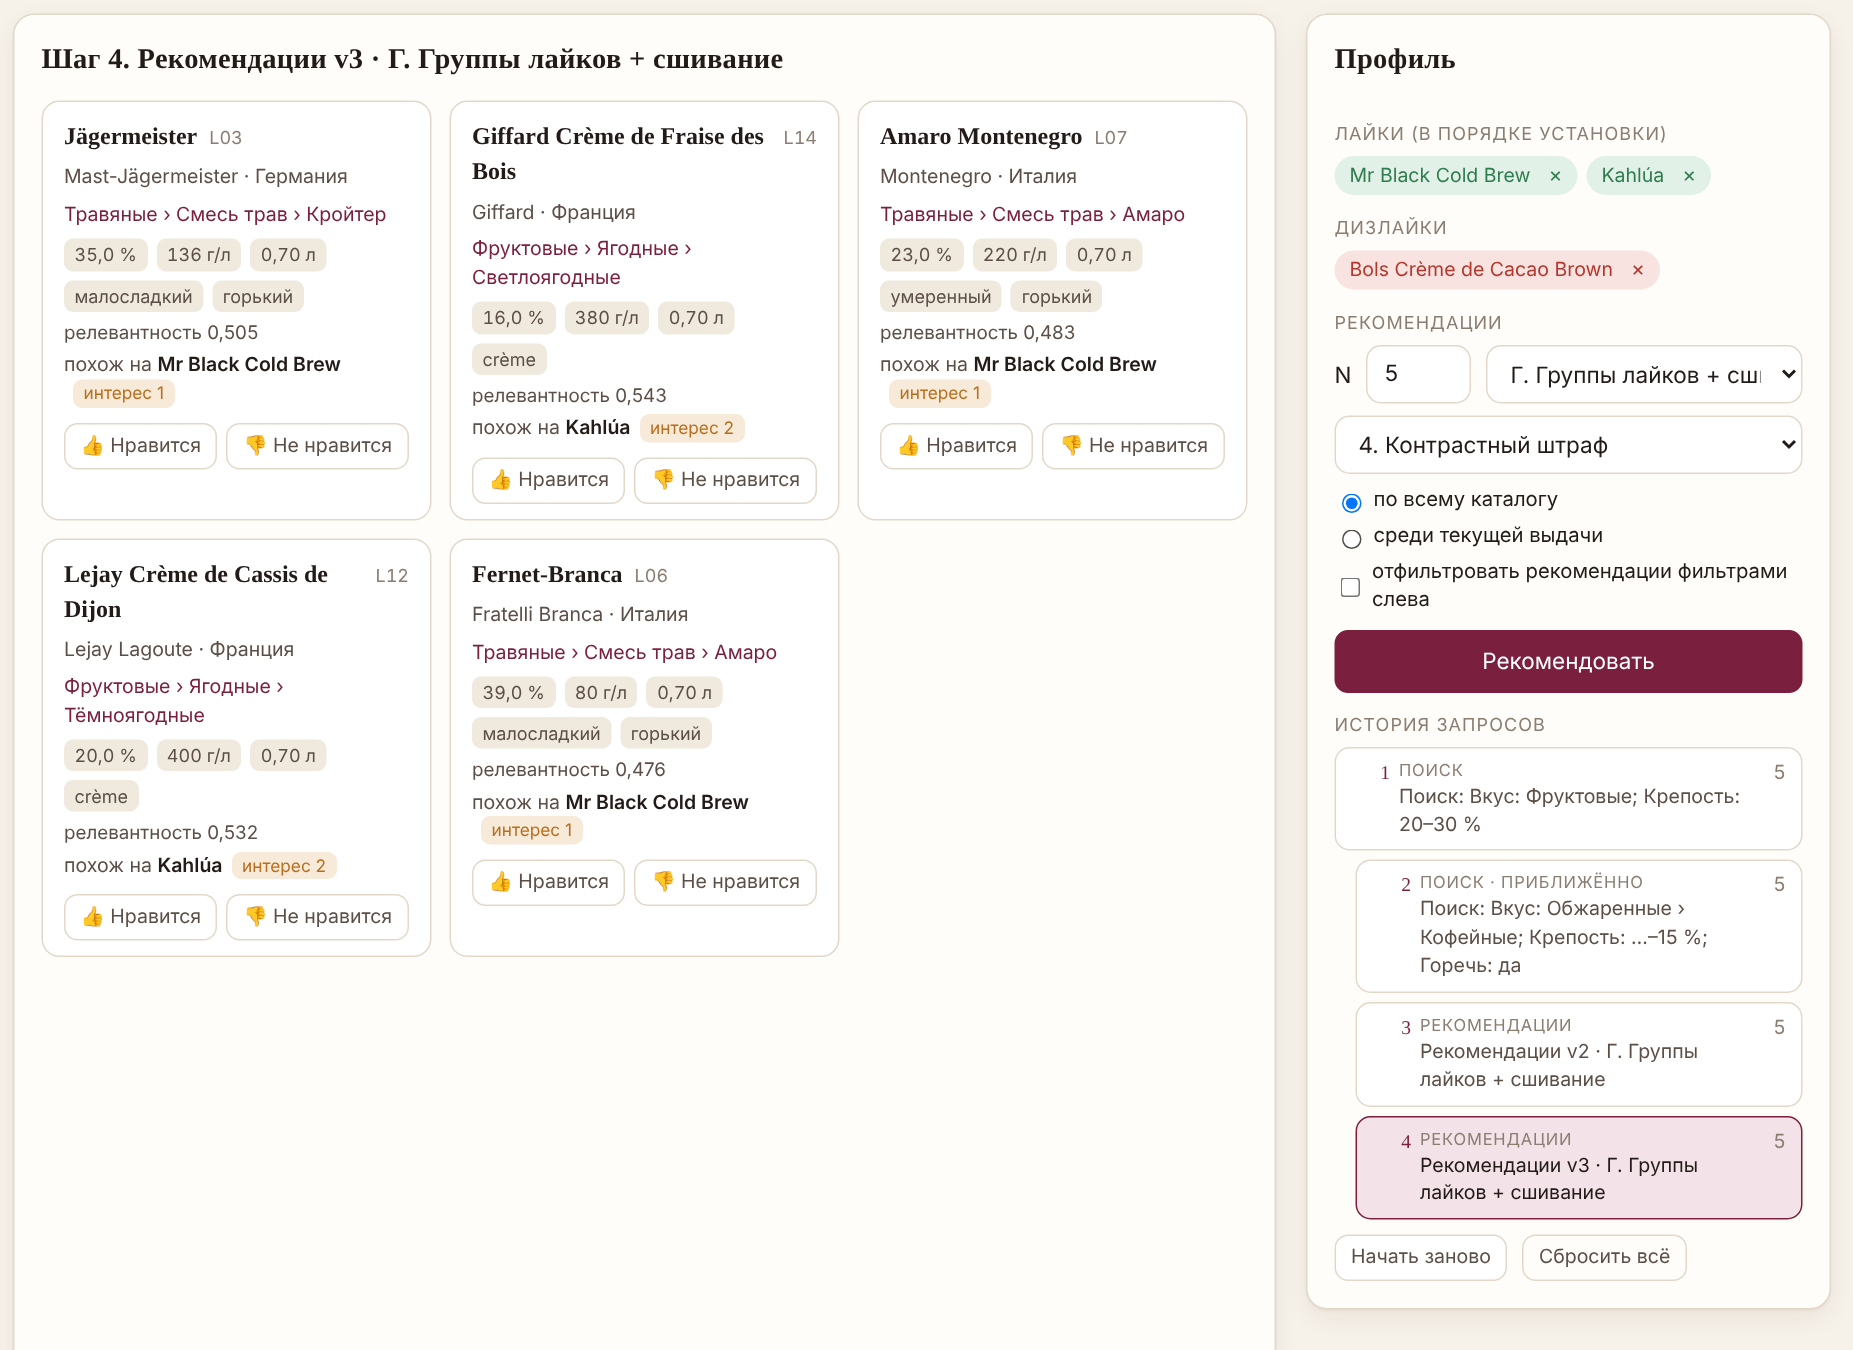
\includegraphics[width=\textwidth]{ui/lr4_recommend.png}
	\caption{Шаги 3--4. Лайки Mr Black и Kahl\'ua из выдачи, дизлайк Cr\`eme de Cacao Brown, рекомендации v3}
	\label{fig:ui_lr4_rec}
\end{figure}

На рисунке~\ref{fig:ui_lr4_refine} рекомендации уточнены фильтром <<сахар не более 300 г/л>>. Объяснения рекомендаций при этом сохранены.

\begin{figure}[H]
	\centering
	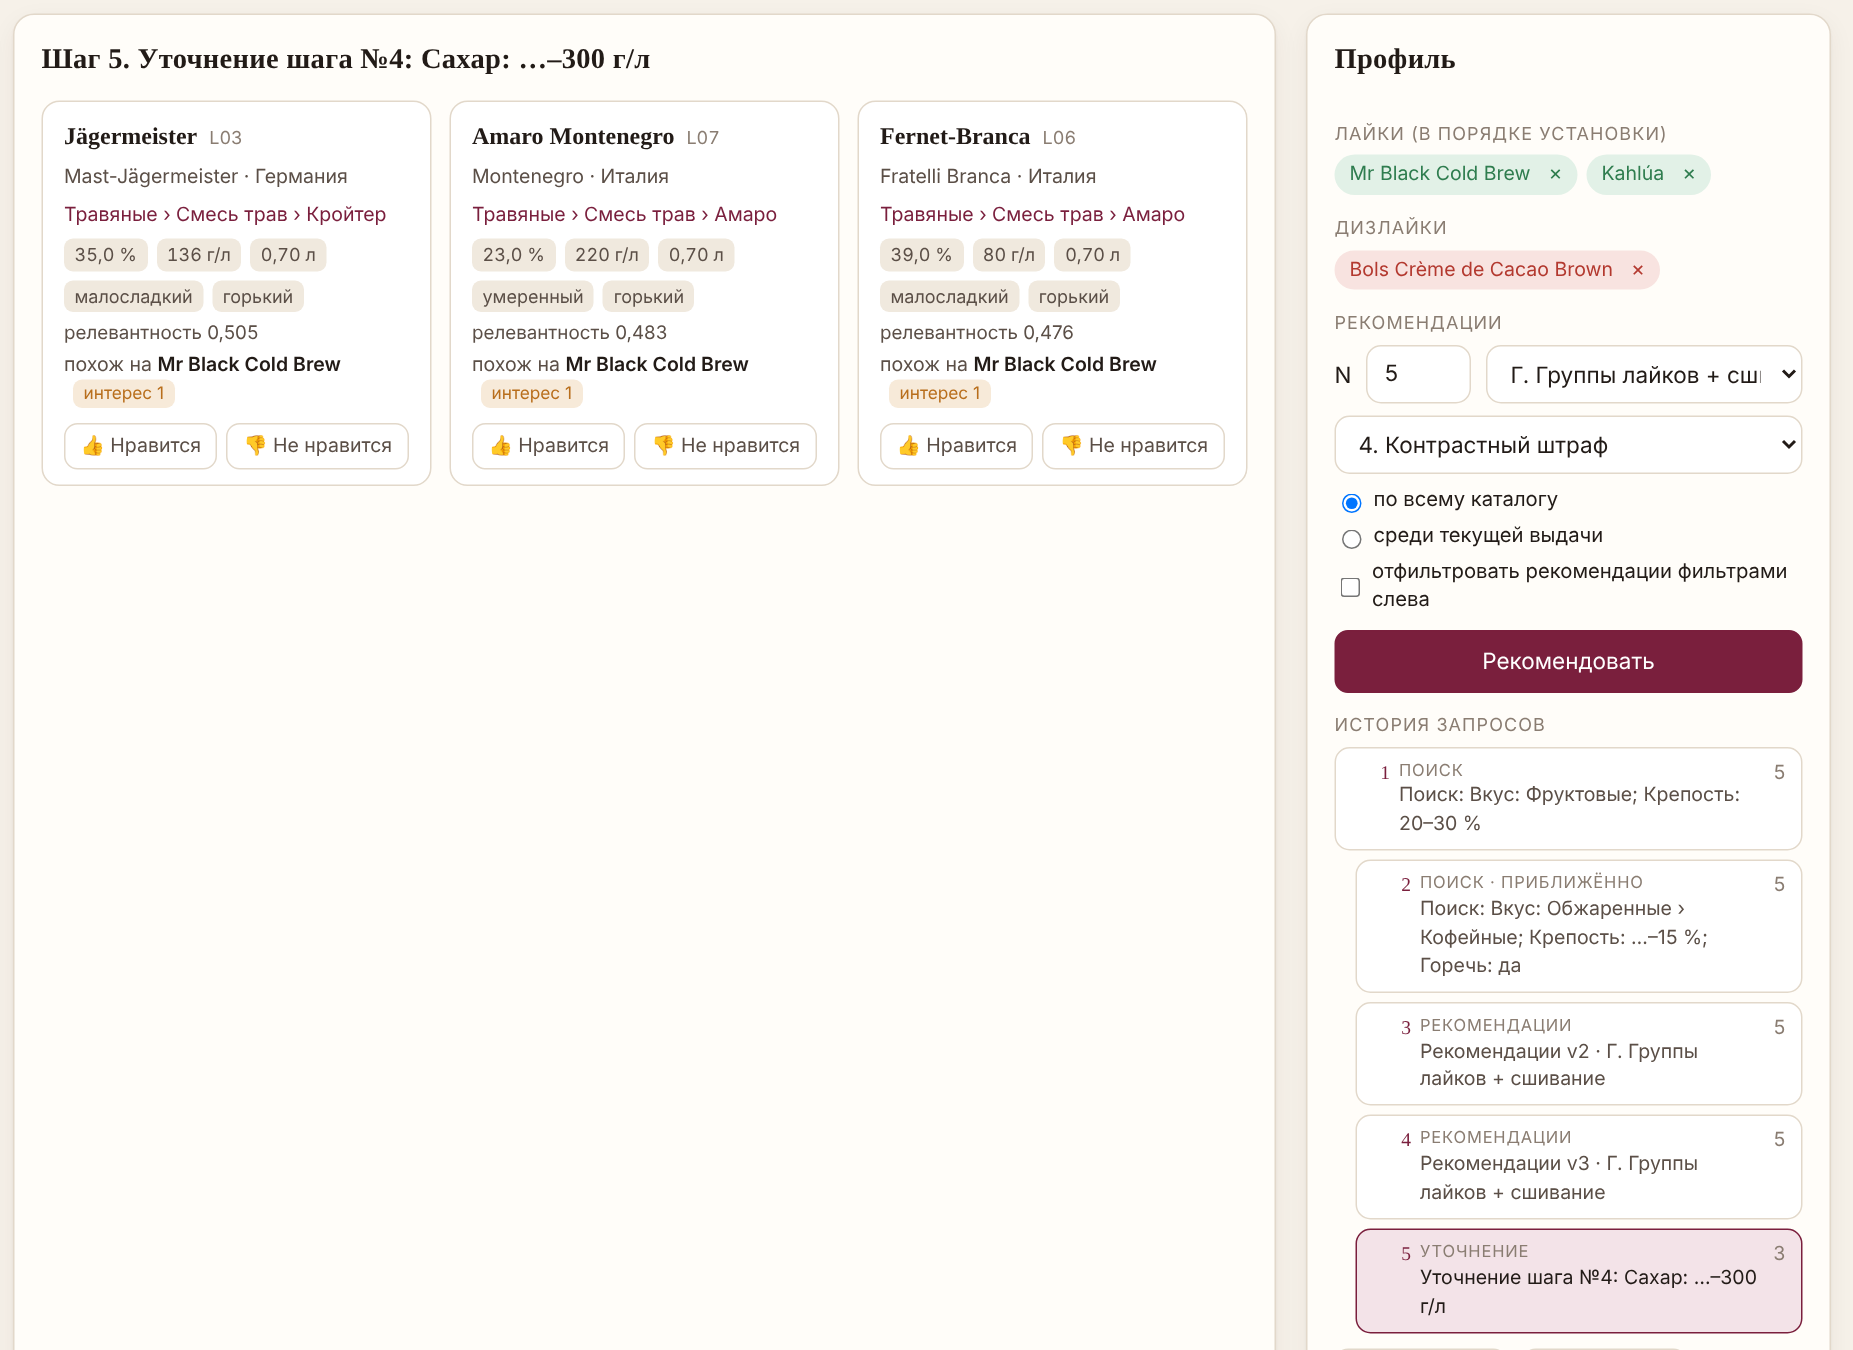
\includegraphics[width=\textwidth]{ui/lr4_refine.png}
	\caption{Шаг 5. Уточнение рекомендаций фильтром <<сахар не более 300 г/л>>. Объяснения рекомендаций сохранены}
	\label{fig:ui_lr4_refine}
\end{figure}

На рисунке~\ref{fig:ui_lr4_rec_filters} рекомендации построены по всему каталогу и отфильтрованы условиями <<Франция, крепость от 30\,\%>>.

\begin{figure}[H]
	\centering
	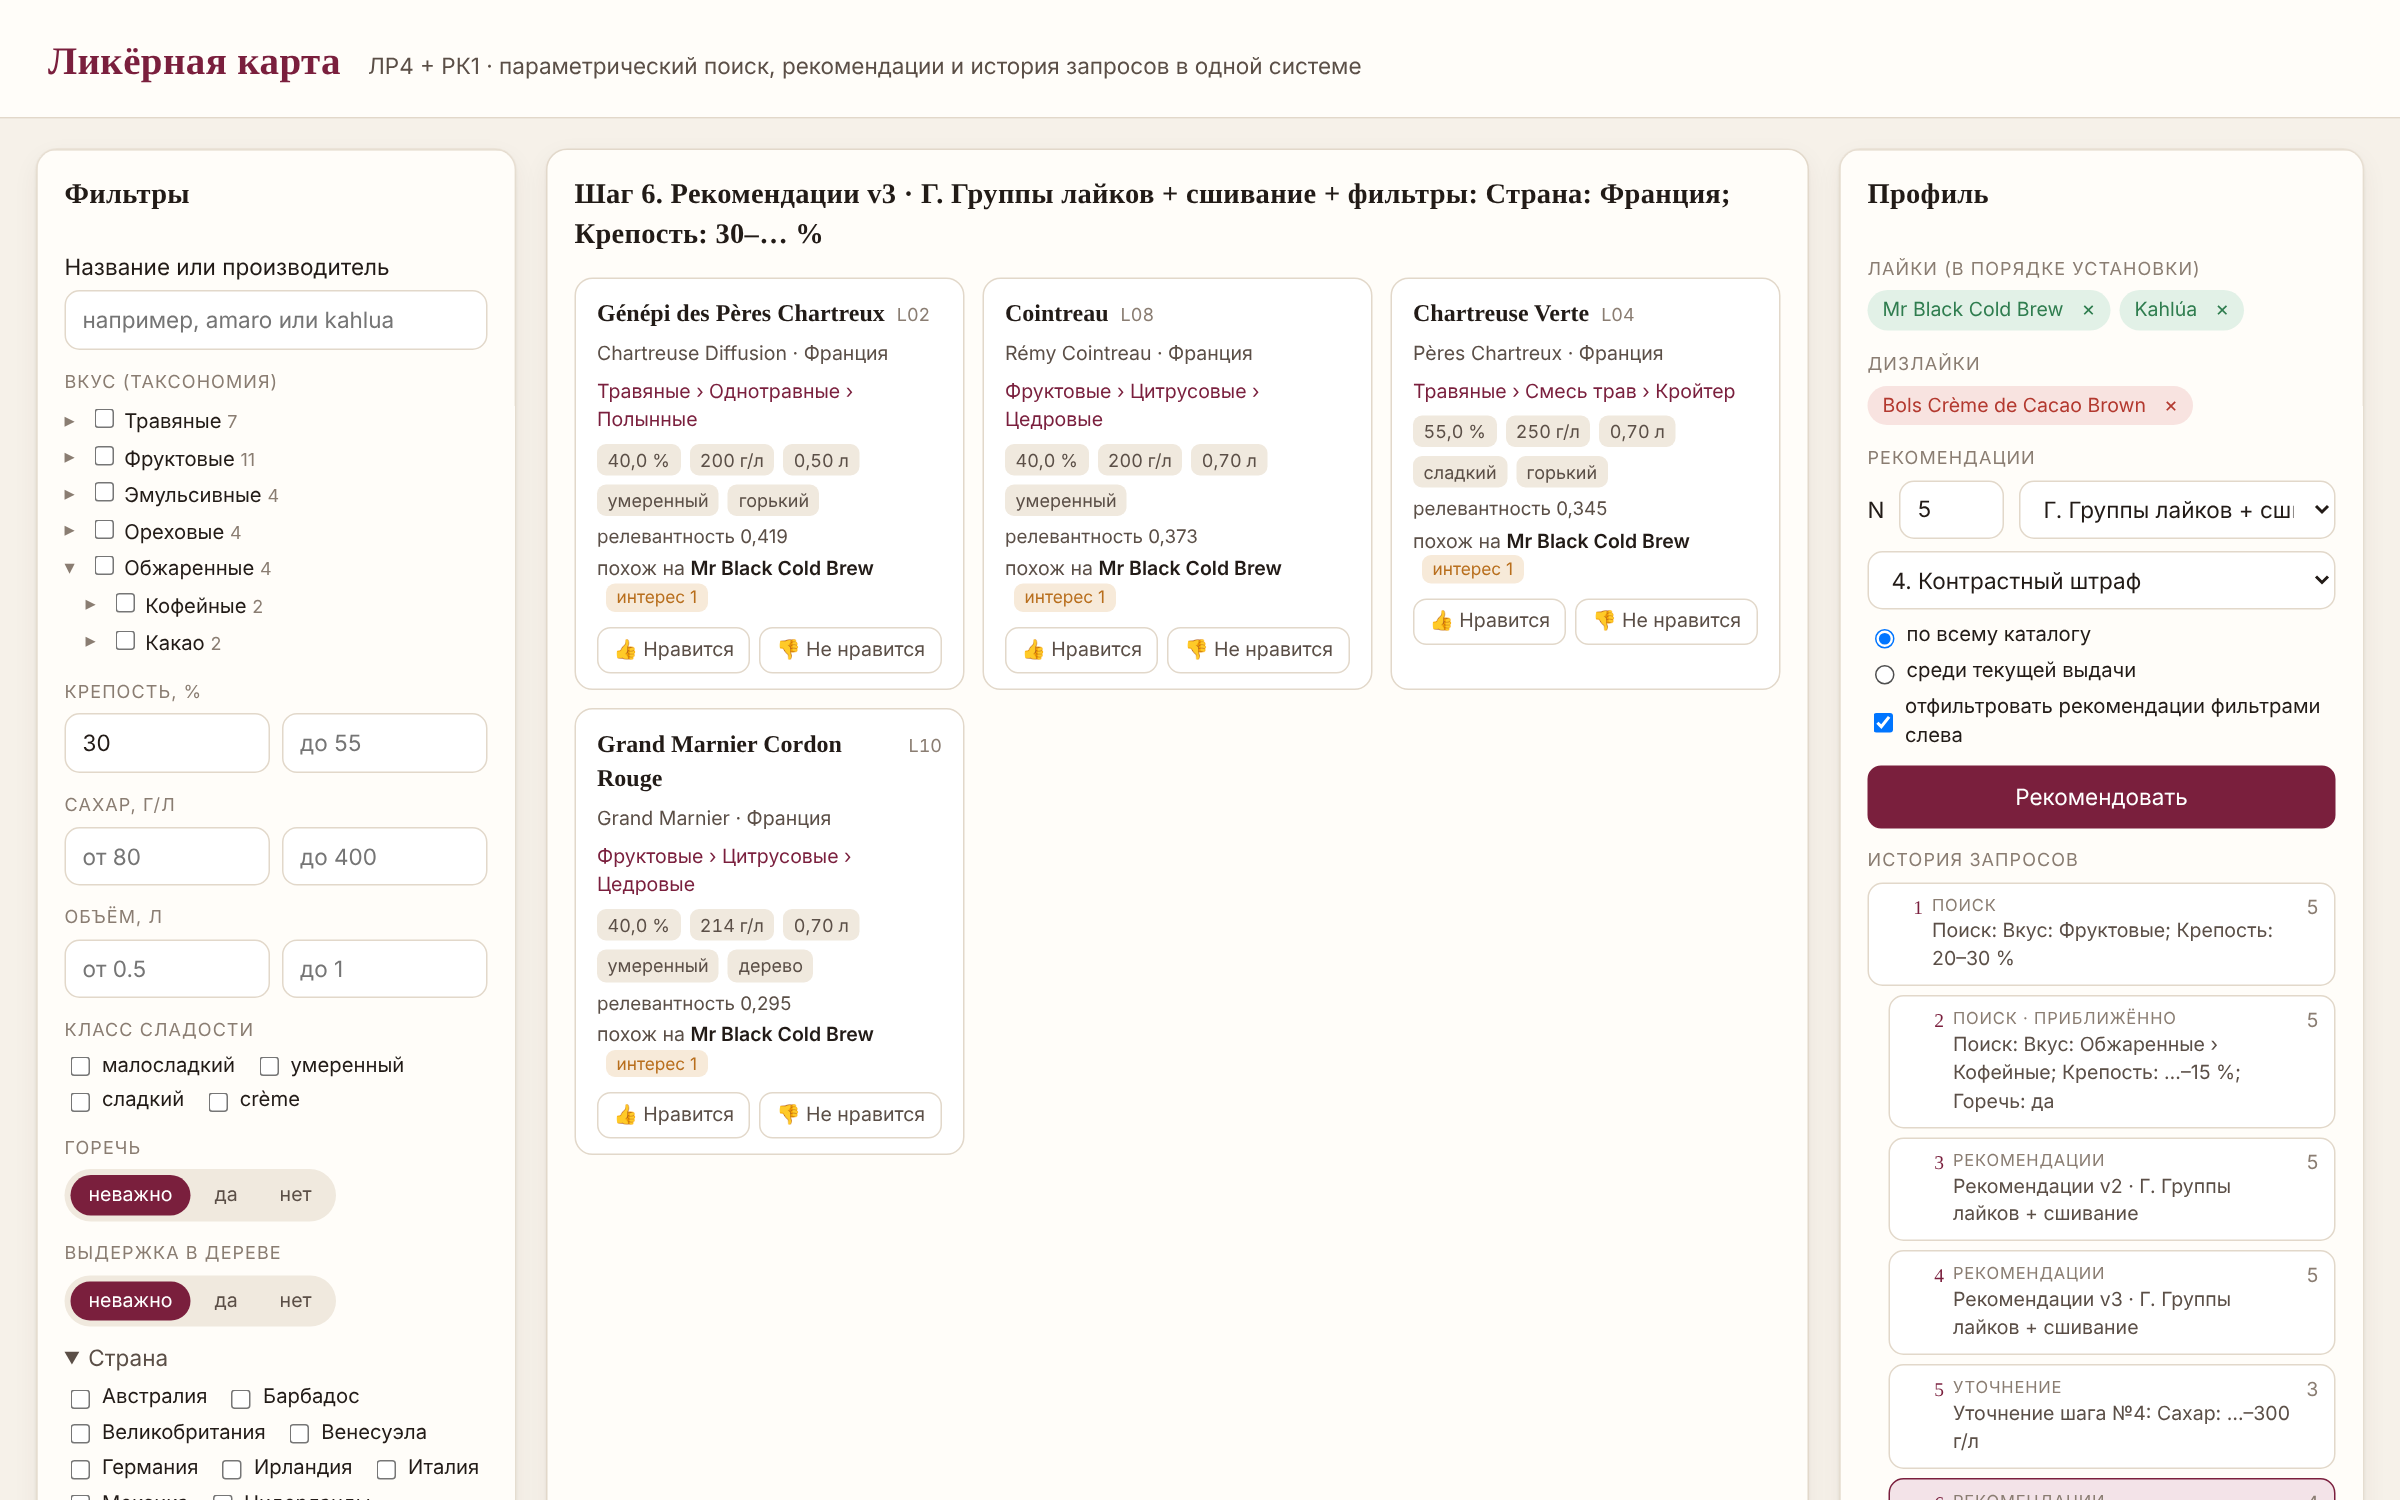
\includegraphics[width=\textwidth]{ui/lr4_rec_filters.png}
	\caption{Шаг 6. Рекомендации по всему каталогу, отфильтрованные условиями <<Франция, крепость от 30\,\%>>}
	\label{fig:ui_lr4_rec_filters}
\end{figure}

На рисунке~\ref{fig:ui_lr4_history} показан возврат к первому шагу через историю. Выдача и форма фильтров восстановлены.

\begin{figure}[H]
	\centering
	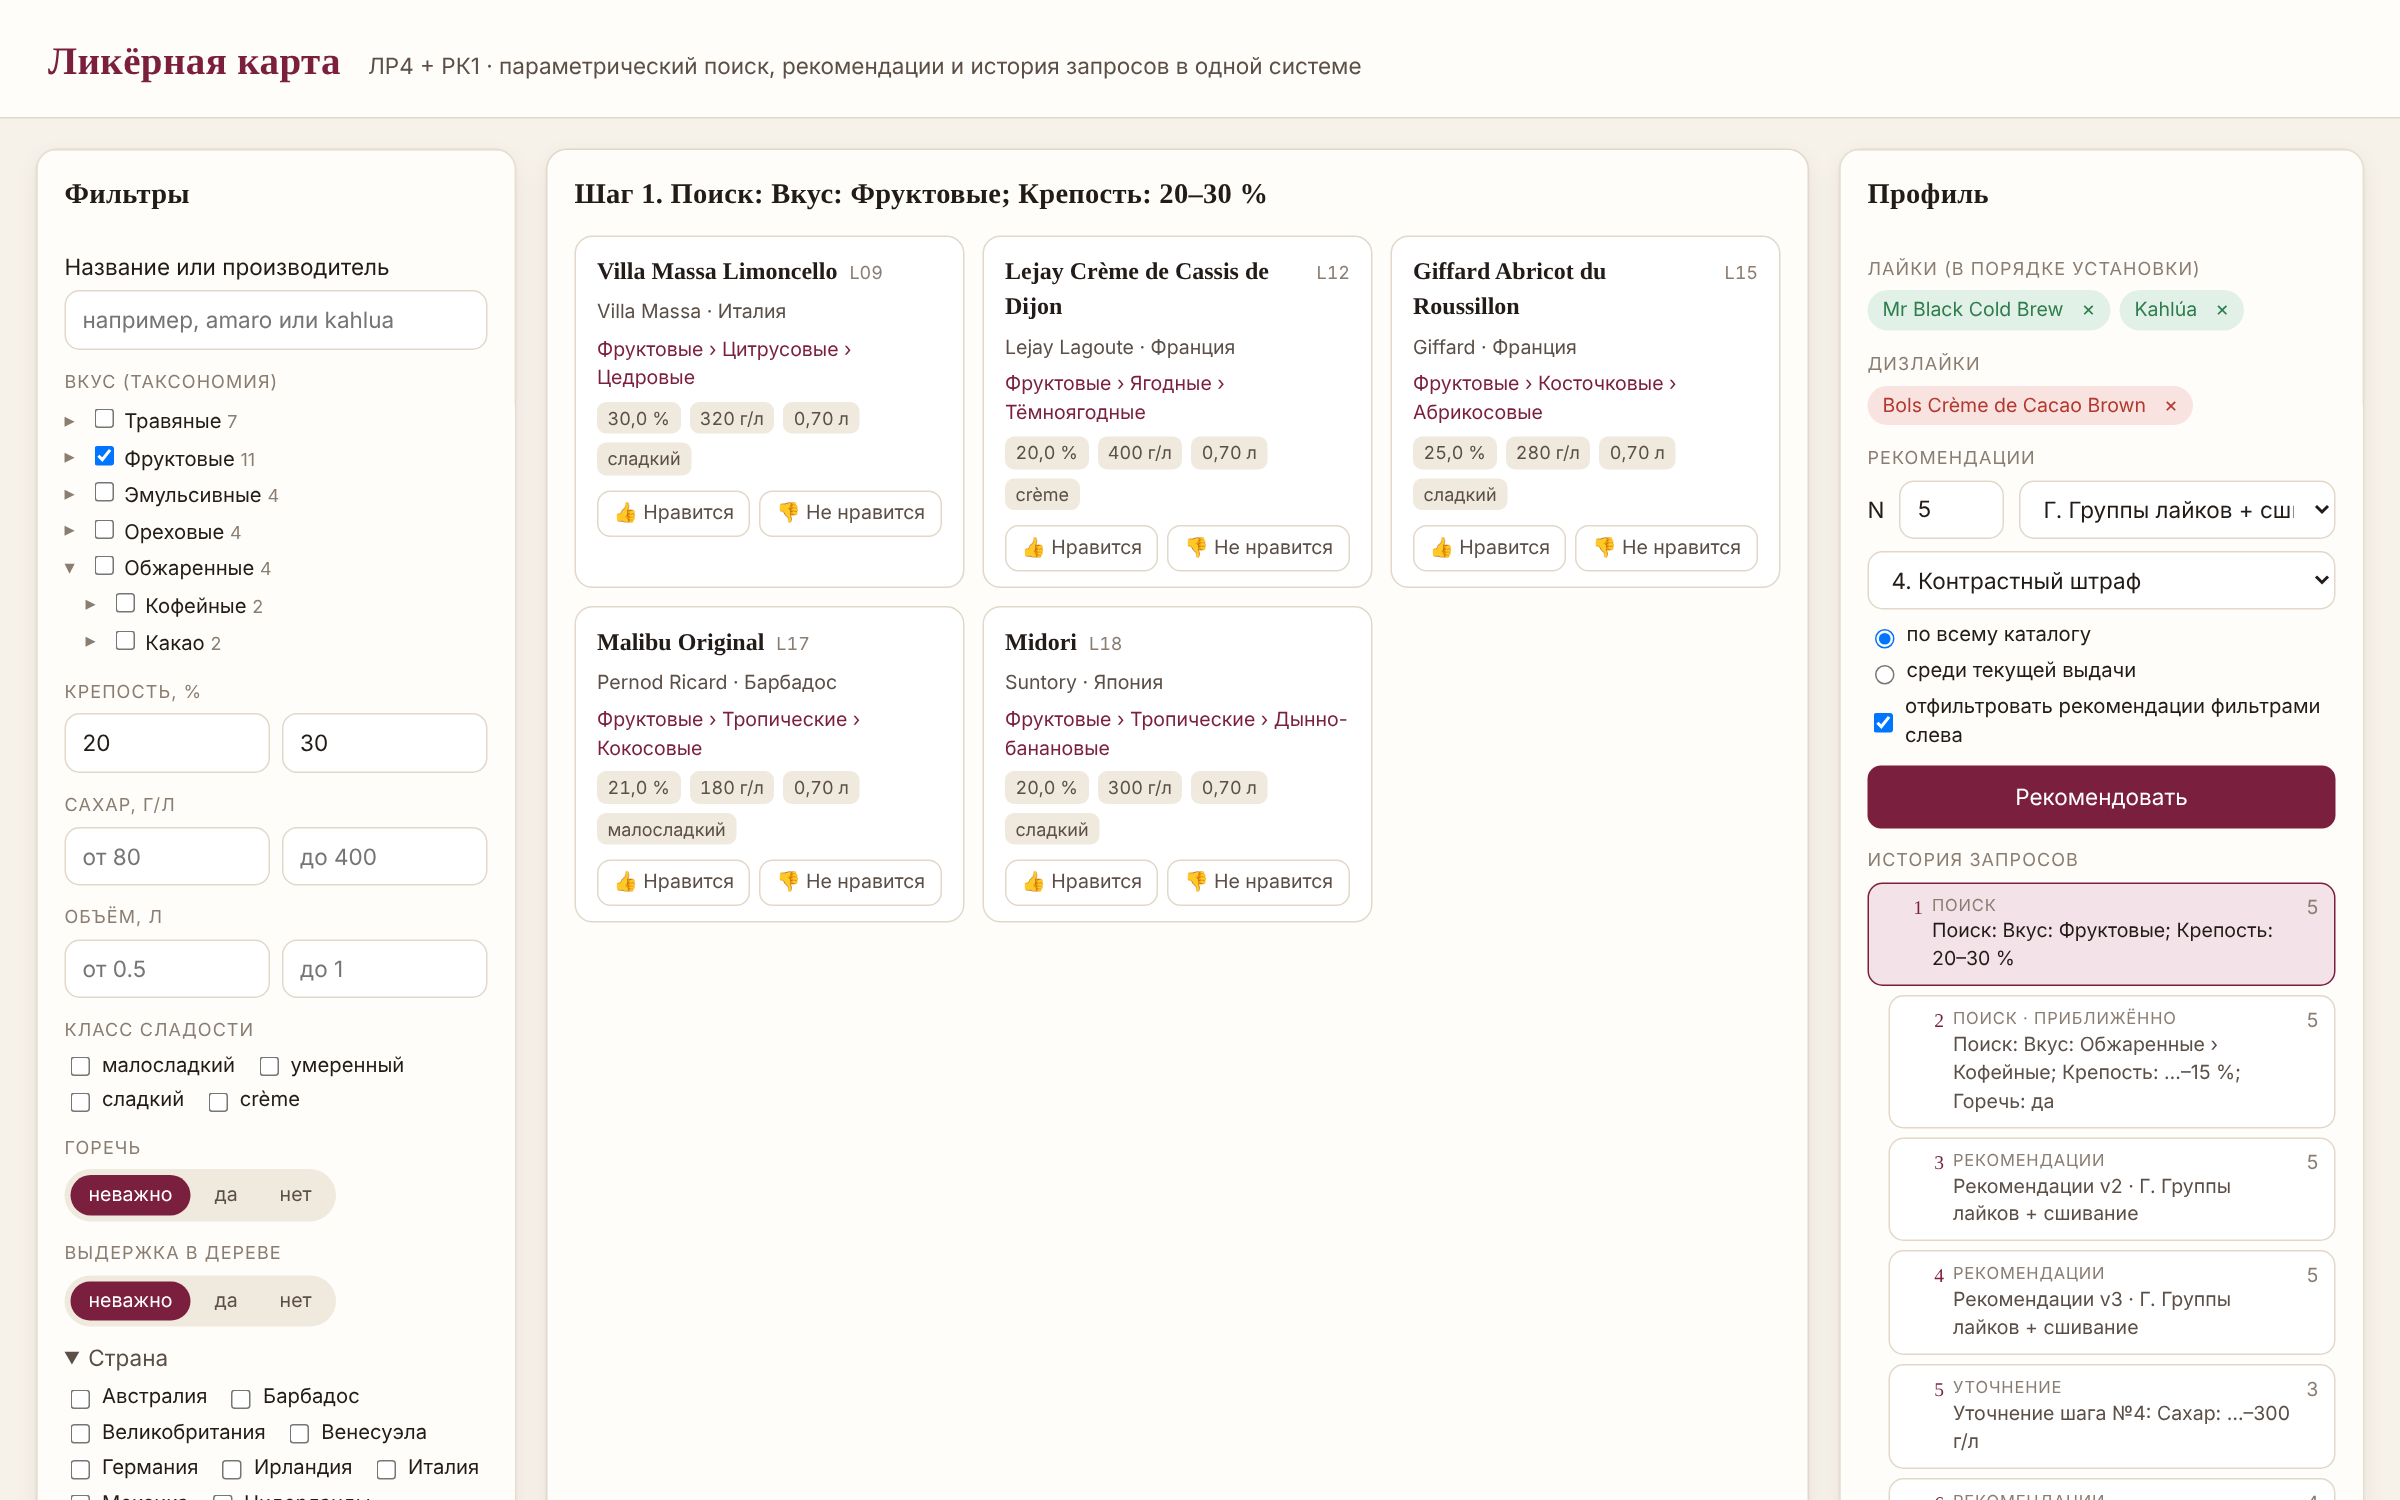
\includegraphics[width=\textwidth]{ui/lr4_history.png}
	\caption{Возврат к шагу 1 через историю. Восстановлены выдача и форма фильтров}
	\label{fig:ui_lr4_history}
\end{figure}

Ввод проверяется на сервере, и все ошибки возвращаются одним списком. Пример показан на рисунке~\ref{fig:ui_lr4_errors}.

\begin{figure}[H]
	\centering
	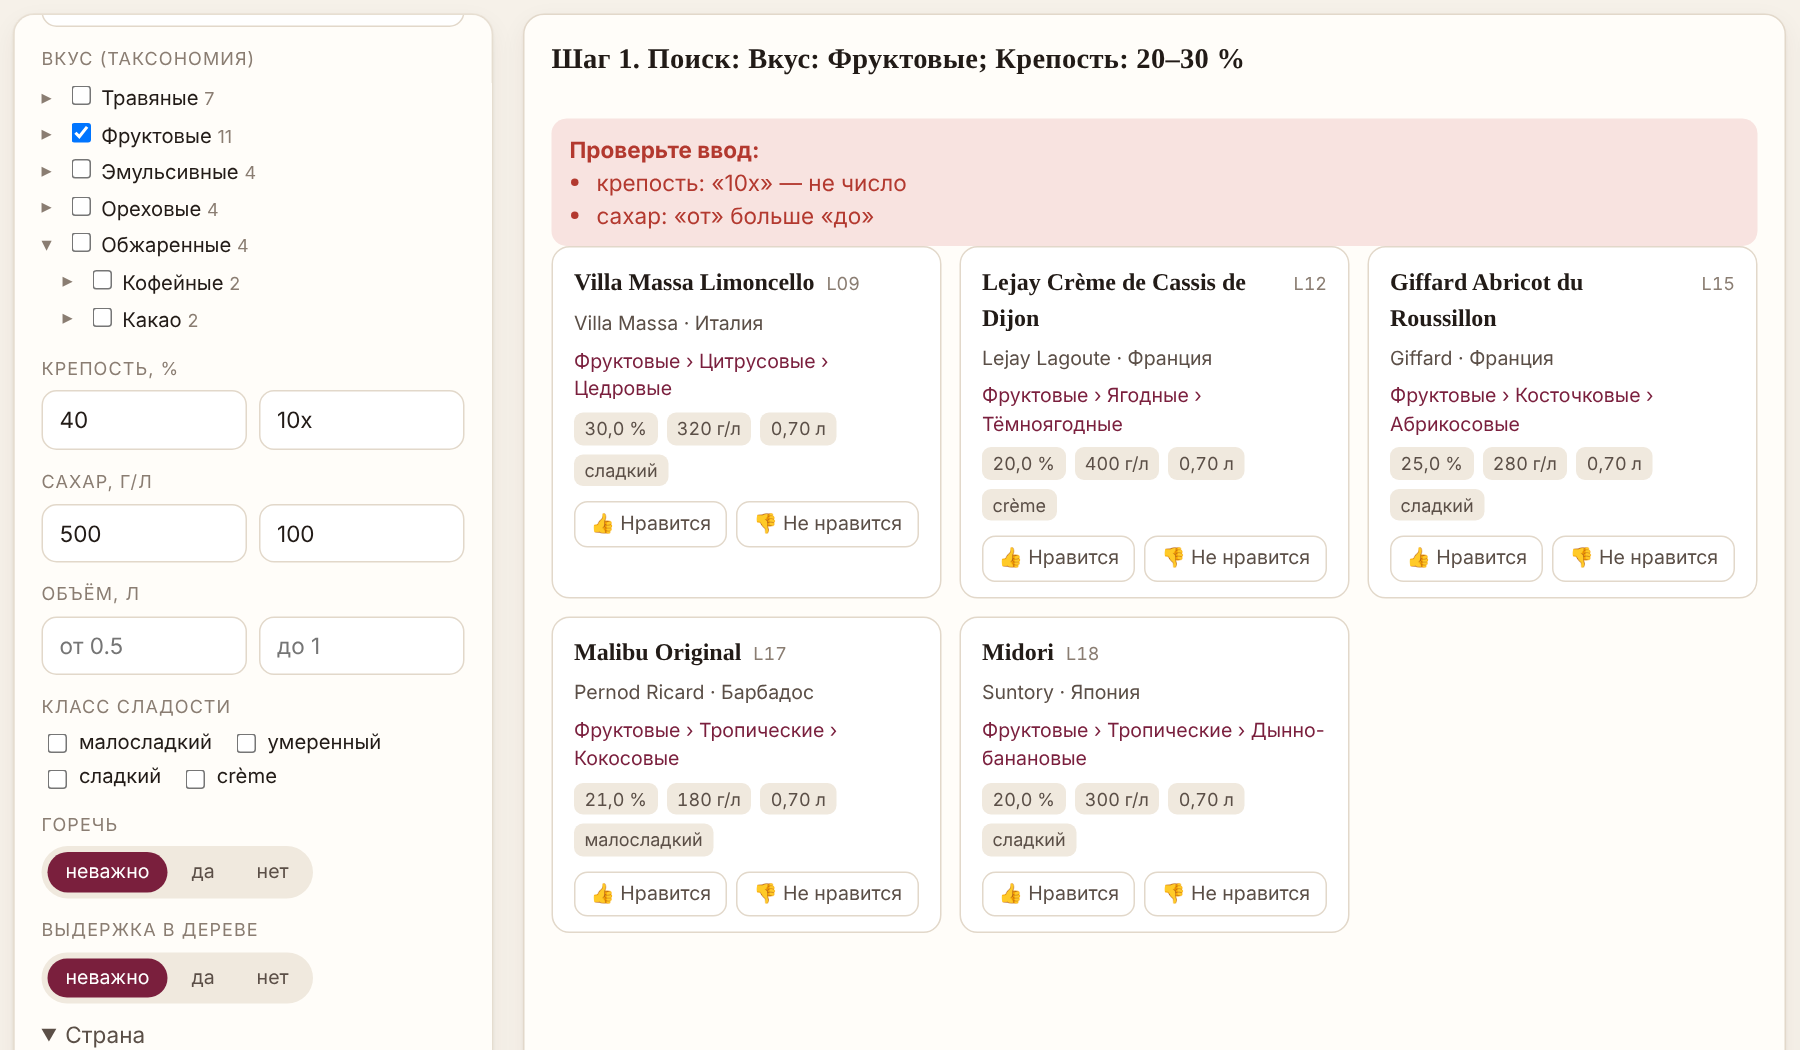
\includegraphics[width=\textwidth]{ui/lr4_errors.png}
	\caption{Ошибки ввода. Все нарушения формы показаны одним списком}
	\label{fig:ui_lr4_errors}
\end{figure}

\section*{Выводы}
\addcontentsline{toc}{section}{Выводы}

Реализован параметрический поиск по десяти фильтрам всех типов признаков с проверкой ввода. Для пустой выдачи выбрана функция полезности. Она восстанавливает задуманный объект в первой пятёрке во всех 179 тестовых сценариях, а ослабление фильтров --- только в 70\,\%. Ослабление используется как подсказка пользователю. Поиск и рекомендации ЛР3 объединены в систему с общим интерфейсом, сессионным профилем, фильтрацией рекомендаций по функции полезности~\eqref{eq:rk1_score} и историей шагов. К любому шагу можно вернуться для уточнения или начать работу заново.
